\chapter{State of the art}
\label{ch:state-of-art}

Automated plant phenotyping is now increasingly prevalent in both research and education, driven by low-cost sensors, single-board computers and open-source analysis pipelines \parencite{pieruschka2019phenotyping}. This chapter first reviews the main platform families and related technologies, then positions the PhenoHive project within that field.

\section{Commercial and research phenotyping platforms}

At the higher end of the market, commercial phenotyping systems such as LemnaTec and Phenobox provide fully automated, high-throughput measurements of plant growth and physiological responses (Figure~\ref{fig:reference-collage}). These platforms combine multispectral imaging, detailed environmental control and integrated analysis pipelines. They are mainly designed for research institutions, where high cost is justified by throughput and tight experimental control. For teaching programs and individual researchers however, they are usually out of reach because of cost and space requirements.

In the mid-tier and research sector, open-source greenhouse-monitoring platforms provide modular sensor integration, time-series storage and image-analysis workflows that can be assembled and customized. Representative examples include FarmBot \parencite{farmbot} (an open-source precision agriculture robot) and community-maintained sensor-logging stacks built on InfluxDB and Grafana. Many of these systems run on Raspberry Pi or similar single-board computers, which makes distributed low-cost deployment realistic. Near-continuous plant monitoring with affordable hardware is increasingly feasible, and educational platforms have begun adopting this model.

\begin{figure}[H]
    \centering
    \begin{subfigure}[b]{0.3\textwidth}
        \centering
        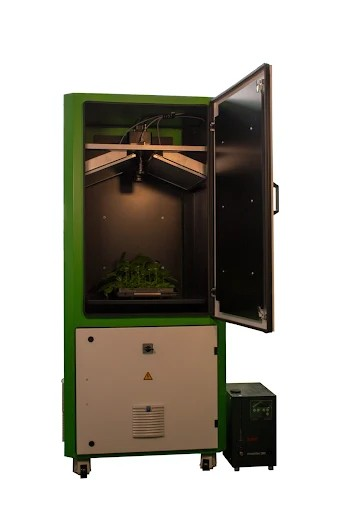
\includegraphics[width=\textwidth]{Images/Lemnatec}
        \caption{LemnaTec High-Throughput Greenhouse System.}
        \label{fig:lemnatec}
    \end{subfigure}
    \hfill
    \begin{subfigure}[b]{0.3\textwidth}
        \centering
        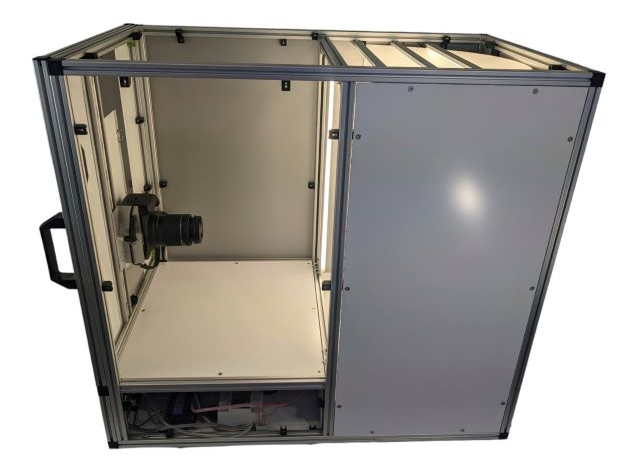
\includegraphics[width=\textwidth]{Images/phenobox}
        \caption{PhenoBox Research Enclosure.}
        \label{fig:phenobox}
    \end{subfigure}
    \hfill
    \begin{subfigure}[b]{0.3\textwidth}
        \centering
        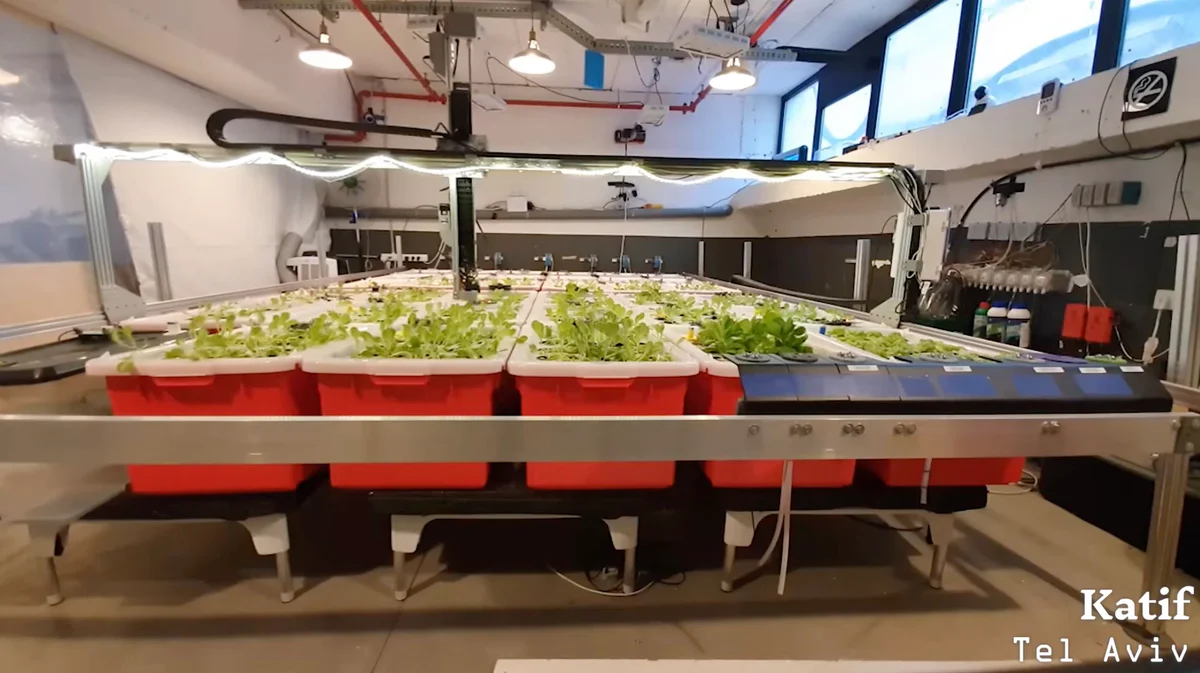
\includegraphics[width=\textwidth]{Images/farmbot}
        \caption{FarmBot Open-Source Precision Agriculture Robot.}
        \label{fig:farmbot}
    \end{subfigure}
    \caption[Commercial, Open-Source and Educational Phenotyping Reference Systems]{Representative phenotyping platforms across market/price tiers. LemnaTec \parencite{lemnatec-solutions, vienna-scientific-phenobox} and PhenoBox are commercial high-throughput systems that are designed for research institutions. These emphasize throughput and total environmental control. FarmBot \parencite{farmbot} is a community-maintained open-source robot that illustrates the modular and affordable end of the spectrum. All three contrast with the portable, educational focus of PhenoHive .}
    \label{fig:reference-collage}
\end{figure}

\section{Educational platforms for plant biology}

In academic settings, plant physiology and botany courses often depend on manual measurements, shared greenhouse facilities, or pre-recorded datasets. Several institutions have developed open-source platforms for continuous plant monitoring in teaching and research contexts. Phenotiki \parencite{minervini2017phenotiki} is an example of a Raspberry Pi-based platform for image-based phenotyping of rosette plants, designed to lower the barrier to entry for laboratory use. The Growth Monitor Pi (GMPi) \parencite{grindstaff2019gmpi} similarly targets affordable remote monitoring of plant growth in facilities, using single-board computers to enable continuous observation without dedicated infrastructure. The diversity of these approaches reflects different pedagogical goals. Some platforms emphasize instrumentation, while others prioritize biological observation and interpretation. The PhenoHive project follows the second approach, where technology is a tool for observation rather than the primary subject of study.

Autonomous monitoring addresses a timescale mismatch. The physiological processes students are asked to observe acclimation responses, growth allocation, VPD-driven stomatal behavior unfold over days and weeks, not laboratory hours. Continuous sensors also remove the greenhouse bottleneck, letting twenty groups run parallel experiments with different conditions simultaneously. The reduction in collection overhead shifts student attention from measurement logistics toward experimental design and biological interpretation.
The biological signals that make this extended monitoring valuable are grouped into four measurement domains (Table~\ref{tab:phenotyping-metrics-interpretation}).
\begin{table}[H]
\centering
\caption[Core Phenotyping Metrics and Physiological Interpretation]{Core metrics used in plant phenotyping and their physiological interpretation. Environmental, light, mass and morphology signals are not interpreted independently; they are jointly used to reason about transpiration, photosynthesis and growth dynamics over time.}
\label{tab:phenotyping-metrics-interpretation}
\footnotesize
\setlength{\tabcolsep}{5pt}
\renewcommand{\arraystretch}{1.2}
\begin{tabularx}{\textwidth}{|P{2.5cm}|X|X|}
\hline
\textbf{Measurement domain} & \textbf{Primary metrics} & \textbf{Physiological interpretation} \\
\hline
Environment & Air temperature, relative humidity, vapor pressure deficit (VPD) & Transpiration behavior, stomatal context, stress exposure \\
\hline
Light & Intensity and spectral composition & Photosynthetic context, acclimation response \\
\hline
Mass & Pot mass trend and short-term variation & Water-balance dynamics, biomass accumulation trajectory \\
\hline
Imaging & Projected leaf area, canopy color, shape descriptors & Growth progression, visual stress signatures \\
\hline
\end{tabularx}

\vspace{0.4em}
{\footnotesize Cross-cutting quality dimensions: temporal continuity, sampling interval and data quality (missing values, outliers, drift).}
\end{table}
PhenoHive is specifically designed for this teaching context, where the primary goal is pedagogical understanding and where stations may be deployed in diverse, uncontrolled environments such as student homes. Table~\ref{tab:platform-landscape-comparison} positions PhenoHive within this field.
\begin{table}[H]
\centering
\caption[Phenotyping Platform Families Comparison]{Comparison of plant phenotyping platform families across cost, throughput, modalities, deployment context and teaching access. Commercial systems maximize automation, while open-source and educational platforms prioritize flexibility and affordability.}
\label{tab:platform-landscape-comparison}

\footnotesize
\setlength{\tabcolsep}{4pt}
\renewcommand{\arraystretch}{1.25}
\rowcolors{2}{gray!8}{white}
\begin{tabularx}{\textwidth}{P{2.6cm}Y Y Y Y}
\textbf{Criterion} & \textbf{Commercial} & \textbf{Open-source} & \textbf{Educational} & \textbf{PhenoHive (this thesis)} \\
\hline
Cost & High & Moderate & Low & Low ($\sim$€137/unit) \\
Throughput & Very high & Medium & Low & Low (1 plant/station) \\
Main modalities & RGB, multispectral, thermal, mass, climate, often gas exchange & RGB, multispectral, thermal, mass, optional custom sensors & RGB, mass, basic climate, optional light/humidity add-ons & Temp./humidity, 14-channel spectral (calibrated), mass, RGB camera \\
Deployment context & Controlled greenhouse/chamber, dedicated server, high maintenance & Lab/greenhouse, local server or SBC, moderate integration effort & Desk or small enclosure, minimal infrastructure & Student home or desk; single USB supply; Tailscale overlay \\
Typical users & Industry breeding and research centers & Research labs and student projects & Course cohorts and teaching labs & LBIR1251 student groups ($\sim$20 parallel stations) \\
Teaching accessibility & \textit{Low} & \textit{Moderate} & \textbf{High} & \textbf{High} \\
\end{tabularx}
\rowcolors{2}{}{}

\vspace{0.5em}
{\footnotesize Synthesis based on literature and prior PhenoHive theses \parencite{goffinet2024, colinet2025}. PhenoHive sits in the educational cost tier but targets open-source-tier sensing quality through laboratory-validated sensors.}
\end{table}

\section{Sensor integration and measurement strategy}

Sensor selection and integration demonstrate a recurring trade-off between price and precision. High-end phenotyping platforms often integrate many sensors and cameras, which provides multispectral, thermal and morphological data at the same time. This completeness comes with higher complexity, cost and data volume. Educational platforms usually favor a more focused approach, selecting a smaller set of sensors that directly serve learning objectives.

Four variables have the most direct pedagogical value for plant physiology. Spectral light quality and illuminance drive photosynthesis and control developmental responses through phytochrome \parencite{franklin2005phytochromes}. Air temperature and relative humidity jointly determine vapor pressure deficit, which governs stomatal conductance and evapotranspiration \parencite{allen1998fao}. Continuous pot mass provides a slow, integrating water-balance signal; combined with camera images it traces biomass accumulation along two independent lines of evidence.

In many existing platforms, sensor choices reflect availability and budget constraints more than strict pedagogical optimization. In the PhenoHive project's sequence, \textcite{goffinet2024} and \textcite{colinet2025} established a baseline that made continuous environmental and growth observation feasible in an educational context. Their work also showed which variables needed stronger characterization in later iterations.

The VPD and the spectral band ratio carry the most direct pedagogical relevance of the four. Both need precisely calibrated sensors which is what drives the sensor selection in Chapter~\ref{ch:data-acquisition}. Not only that but with 20 groups running in parallel, the measurements also have to stay consistent and comparable. If they aren't, this means that no group can trust the conclusions it draws from its own experiment.

\section{Synthesis of previous PhenoHive theses}

The two previous PhenoHive theses advanced the platform in concrete, distinct steps (Figure~\ref{fig:phenohive-timeline}). \textcite{goffinet2024} established the continuous-monitoring feasibility on DietPi, modularised the codebase and provided the first automated deployment pipeline with a self-hosted visualization stack. \textcite{colinet2025} upgraded the hardware, improved the image-analysis pipeline with shadow detection, migrated the visualization infrastructure to an online server, and added first-generation environmental sensors (a resistive soil moisture probe and a photoresistor). Considered together, these works demonstrate a clear progression in platform maturity. What they also reveal is the gap between having a sensor \emph{connected} and having a signal that is \emph{metrologically grounded} and \emph{physiologically informative}. The soil moisture index cannot substitute for air humidity in VPD calculations, and a photoresistor cannot discriminate the spectral bands that drive phytochrome-mediated plant responses.

This review of the state of the art in plant phenotyping platforms, and of the PhenoHive project's trajectory, all show that for a platform to be effective, it must be reliable, accurate and pedagogically relevant. Also, keeping the platform easily maintainable and extensible is critical for its long-term success in an educational setting. The next chapters will therefore cover detail how the current iteration of PhenoHive addresses these requirements through sensor calibration, software architecture refactor and deployment strategy improvements.


\begin{figure}[H]
\centering
\begin{tikzpicture}[
    milestone/.style={draw, rounded corners, align=left, text width=3.8cm, inner sep=5pt, font=\footnotesize},
    title/.style={font=\bfseries\footnotesize, align=center},
    flowarrow/.style={-{Latex[length=2.3mm]}, thick}
]
% Timeline axis
\draw[thick] (0,0) -- (12,0);

% Milestone markers
\fill (1,0) circle (1.6pt);
\fill (6,0) circle (1.6pt);
\fill (11,0) circle (1.6pt);

% Direction arrows
\draw[flowarrow] (1.6,0) -- (5.4,0);
\draw[flowarrow] (6.6,0) -- (10.4,0);

% Titles above markers
\node[title] at (1,0.55) {2024: Goffinet};
\node[title] at (6,0.55) {2025: Colinet};
\node[title] at (11,0.55) {Current thesis};

% Description boxes below the timeline
\node[milestone, anchor=north] at (1,-0.35) {
\textbullet\ DietPi OS migration + automated SD setup.\\
\textbullet\ Code modularisation (type hints, docstrings).\\
\textbullet\ Rolling-median filter for mass tracking.\\
\textbullet\ Local InfluxDB/Grafana via RPi hotspot.
};

\node[milestone, anchor=north] at (6,-0.35) {
\textbullet\ RPi Zero W $\rightarrow$ Zero 2W hardware upgrade.\\
\textbullet\ PlantCV 4.6 + shadow detection (DSC).\\
\textbullet\ Soil moisture probe + photoresistor added.\\
\textbullet\ InfluxDB/Grafana migrated to UCLouvain VM.\\
\textbullet\ Compact 3D-printed enclosure.
};

\node[milestone, anchor=north] at (11,-0.35) {
\textbullet\ Modular architecture refactor (core/sensors/ui/vision).\\
\textbullet\ SHT35 \& TCS3448 lab calibration (WELCOME lab).\\
\textbullet\ Local-first persistence + offline replay queue.\\
\textbullet\ Headless onboarding (Comitup) + Tailscale overlay.\\
\textbullet\ Auto-provisioning (Grafana dashboards + accounts).\\
\textbullet\ Metrics-driven framing for pedagogical comparability.
};
\end{tikzpicture}

\vspace{0.4em}
{\footnotesize \textbf{Overall trajectory:} feasibility \& automation $\rightarrow$ hardware upgrade \& image quality \& VM migration $\rightarrow$ modular architecture \& metrological calibration \& operational hardening.}

\vspace{0.2em}
{\footnotesize Scope note: timeline summarizes thesis-level contributions, not full implementation details.}
\caption[Evolution of the PhenoHive Platform]{Evolution of the PhenoHive platform across consecutive theses where each one contributes a distinct step to the maturation of the platform as a whole. From initial feasibility to expanded observation and metrics-driven pedagogical framing.}
\label{fig:phenohive-timeline}
\end{figure}
